\documentclass[]{../../../NoTeX/notex}
\usepackage{../../../NoTeX/notexmacros}
\usepackage[italian]{babel}

\SetKwInput{KwIng}{Input}
\SetKwInput{KwUsc}{Output}
\SetKwFor{Per}{per}{fai}{fine per}
\SetKwIF{Sea}{AltSe}{Altrimenti}{se}{allora}{altrimenti se}{allora}{fine se}

\renewcommand{\sectionname}{Sezione}

\title{\textsc{Analisi e Calcolo Numerico}}
\author{Leonardo Biason}

\renewcommand{\titleheader}{
    {\Large \textbf{\textsc{Sapienza, University of Rome}}}
    \linebreak
    {\large \textsc{Course of Applied Computer Science and Artificial Intelligence (ACSAI)}}
    
    \vspace{0.05cm}
    {\normal \textsc{3rd Year, 2nd Semester}}
    }
\renewcommand{\titlecourse}{Analisi e Calcolo Numerico}
\renewcommand{\titlecover}{../../../Assets/ACN-bg.jpg}
\renewcommand{\titleauthor}{Leonardo Biason}
\renewcommand{\titlesubtitle}{Course taught by prof. Domenico Vitulano}
\renewcommand{\titlefooter}{
    \begin{tabular}{c c c}
        
\includegraphics[height=1.5cm]{../../../Assets/uniroma1.png} & \hspace{2cm} & 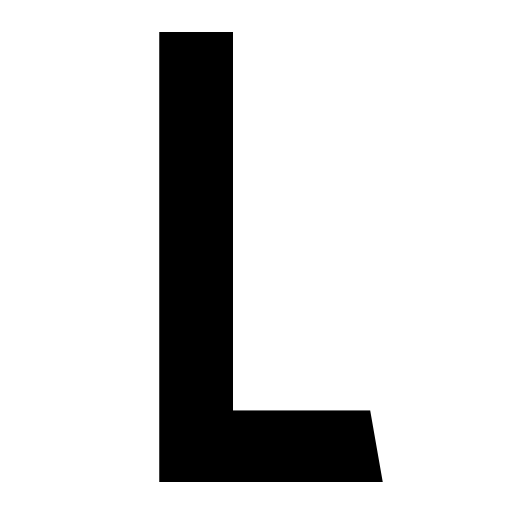
\includegraphics[height=1.5cm]{../../../Assets/icon.png}
    \end{tabular}
}

\begin{document}
    \maincol{HTML}{D06B6B}
    \input{../../../NoTeX/notextitle.tex}

    \vspace{12pt}
\section*{About these notes}

Those notes were made during my three years of university at Sapienza, and \textbf{do not} replace any professor, they can be an help though when having to remember some particular details. If you are considering of using \textit{only} these notes to study, then \textbf{don't do it}. Buy a book, borrow one from a library, whatever you prefer: these notes won't be enough.

\vspace{32pt}
\section*{License}

The decision of licensing this work was taken since these notes come from \textbf{university classes}, which are protected, in turn, by the \textbf{Italian Copyright Law} and the \textbf{University's Policy} (thus Sapienza Policy). By licensing these works I'm \textbf{not claiming as mine} the materials that are used, but rather the creative input and the work of assembling everything into one file.
\nl
All the materials used will be listed here below, as well as the names of the professors (and their contact emails) that held the courses.
\nl
The notes are freely readable and can be shared, but \textbf{can't be modified}. If you find an error, then feel free to contact me via the socials listed in my \href{https://www.leonardobiason.com}{website}. If you want to share them, remember to \textbf{credit me} and remember to \textbf{not} obscure the \textbf{footer} of these notes.

\vspace{32pt}
\section*{Bibliography \texorpdfstring{\&}{&} References}

\begingroup
    \patchcmd{\thebibliography}{\chapter*}{\section*}{}{}
    \renewcommand{\section}[2]{}%
    
    \begin{thebibliography}{9}
        \bibitem{wasa1} TODO
    \end{thebibliography}
\endgroup

\begin{tcolorbox}[colback=Dandelion!25, colframe=Dandelion!50]
    \begin{center}
        The "\textit{Web and Software Architecture}" course was taught in the Winter semester in 2024 by prof. Emanuele Panizzi (\href{mailto:panizzi@di.uniroma1.it}{\texttt{panizzi@di.uniroma1.it}})
    \end{center}
\end{tcolorbox}

I hope that this introductory chapter was helpful. Please reach out to me if you ever feel like. You can find my contacts on my \href{https://www.leonardobiason.com}{website}. Good luck! \nl
Leonardo Biason\\
{\footnotesize \href{mailto:leonardo@biason.org}{$\to$ \texttt{leonardo@biason.org}}}
    \notextoc

    \chapter{Introduzione al calcolo numerico}

Grazie al costante sviluppo dei computers negli scorsi decenni, la comunità scientifica ha avuto modo di usufruire di strumenti di calcolo sempre più precisi e complessi, necessari per risolvere alcuni problemi di vario tipo. Questo sviluppo ha visto anche un cospicuo interesse verso i metodi di calcolo numerico, che permettono di risolvere in modo non-analitico problemi specifici che non sarebbero, altrimenti, risolvibili. Infatti, seppur non esista sempre una soluzione analitica, \textbf{esiste sempre una soluzione numerica} per un modello matematico \textbf{ben posto} e \textbf{condizionato}, che assuma tuttavia certe assunzioni del corrispondente modello fisico.
\nwl
La realtà infatti non è sempre modellabile attraverso semplici formule fisiche: a volte ci sono parecchie variabili da tenere in conto quando si cerca di risolvere un problema, e non è sempre plausibile considerare tutte queste variabili assieme, soprattutto se il problema va risolto senza l'assistenza di un calcolatore. Consideriamo il seguente esempio: un giocatore di golf colpisce una pallina con una certa velocità $U$, e noi vogliamo sapere per quale angolo $\alpha$ la distanza che verrebbe percorsa dalla pallina da golf sarebbe massima prima che quest'ultima tocchi terra.
\nwl
Grazie alla seconda legge di Newton, possiamo calcolare la distanza percorsa dalla pallina, e se trascurassimo la resistenza dell'aria sarebbe abbastanza semplice trovare la soluzione analitica. Tuttavia, considerando questa resistenza, le equazioni del moto si complicano notevolmente, e determinare la soluzione analitica diventa ora impossibile. Tuttavia, la soluzione numerica rimane calcolabile attraverso l'impiego di metodi numerici adatti.
\nwl
È comunque importante considerare anche il tipo di modello utilizzato: in base al modello matematico di partenza e al metodo utilizzato, si possono ottenere risultati diversi. L'importante è saper scegliere il metodo giusto e l'approssimazione migliore del modello.
\nwl
Per il calcolo numerico, la risoluzione di un problema avviene attraverso i seguenti steps:
\begin{itemize}
    \item formulare un \textbf{modello matematico} in base al problema dato, che diventi uno schema per definire il metodo numerico e l'algoritmo di soluzione;
    \item scegliere un \textbf{metodo numerico} che aiuti nella risoluzione del problema;
    \item definire un \textbf{algoritmo} che porti alla soluzione desiderata;
    \item analizzare la \textbf{soluzione numerica} e interpretarla, capendo se quest'ultima sia una valida soluzione o meno. Si dice che una soluzione numerica sia \textbf{accettabile} se e solo se sia possibile \textbf{stimare gli errori} che accompagnano la soluzione stessa.
\end{itemize}

\section{Errori di approssimazione}

Quando si calcola una soluzione numerica, ci sono varie, possibili fonti di errori che possono condizionare il risultato finale. È possibile avere errori di \textbf{misura} (dati dalla precisione dello strumento), \textbf{inerenti} (creati da un'eccessiva semplificazione del modello reale), di \textbf{troncamento} (generati da una discretizzazione del risultato, generalmente presenti quando si usano metodi numerici che richiedono convergenza), e di \textbf{arrotondamento} (creati dalla macchina che performa i calcoli, in quando la precisione è sempre limitata).
\nwl
Ogni computer dispone di un sistema numerico piuttosto primitivo: questo infatti dispone di un sistema \textbf{finito} di numeri, la cui lunghezza è anch'essa \textbf{finita}. Se normalmente, in campi analitici, siamo abituati a pensare con un insieme di numeri infinito (come quello dei numeri reali, $\mathbb{R}$), con i computer, quando si performano calcoli di analisi numerica, si considera un insieme ristretto, detto dei \textbf{numeri macchina} $\mathbb{F}$. Consideriamo ad esempio alcune delle costanti più famose nel mondo matematico: $\pi$, $e$ e $\sqrt{2}$. Noi sappiamo che questi numeri sono irrazionali, e che si espandono all'infinito. Proviamo a chiedere a una macchina di dirci quali sono questi numeri. Eseguendo il seguente script di Python, otterremo il seguente risultato:

\begin{codeblock}{Rounding.py}
    \begin{lstlisting}[language = Python]
import numpy as np
from math import sqrt

print(np.pi, np.e, sqrt(2), sep="\n")\end{lstlisting}
    \vspace{11pt}
    \begin{tcolorbox}[colback = black!95!Periwinkle!90]
        \begin{lstlisting}[style = notexterm]
Out[1]: 3.141592653589793
        2.718281828459045
        1.4142135623730951\end{lstlisting}
    \end{tcolorbox}
\end{codeblock}

Noi sappiamo che in realtà questi numeri si estendono molto più in profondità di quello che ci ha ritornato Python. Infatti:
\begin{itemize}
    \item $\pi = 3,1415926535897932384626433...$;
    \item $e = 2,71828182845904523536...$;
    \item $\sqrt{2} = 1,4142135623730950488...$
\end{itemize}

Qua notiamo già uno dei primi errori che si incontra quando si usa un calcolatore: i numeri sono \textbf{arrotondati} ad una certa cifra. L'arrotondamento genera spesso qualche tipo di errore, ma è necessario che i numeri subiscano una procedura di arrotondamento prima di poter essere usati da un calcolatore, poiché altrimenti non entrerebbero nella memoria di quest'ultimo, che ricordiamo essere limitata.

\begin{definition}{Errore di arrotondamento}
    Definitiamo l'\textbf{errore di arrotondamento} come la \textbf{differenza} tra il \textbf{numero reale} $x \in \mathbb{R}$ e il \textbf{numero macchina} $m \in \mathbb{F}$ corrispondente:
    \[ e_\text{arr} = x - m \]
\end{definition}

Se un calcolatore approssima tutti i numeri alla $D$esima cifra decimale, allora diciamo che l'errore di arrotondamento è compreso nell'\textbf{intervallo} $[-0,5 \cdot 10^{-D}, \; +0,5 \cdot 10^{-D}]$.
\nwl
Riguardo lo scopo di queste note: MATLAB verrà usato durante il corso per implementare certi metodi numerici. Tale linguaggio di programmazione lavora con 15 cifre decimali significative. Fino a quando non verrà introdotto MATLAB tuttavia, verrà usato Python, che ne usa fino a 17 (anche se negli esempi precedenti $\pi$ e $e$ hanno usato solo 15 cifre, probabilmente a causa del pacchetto \verb|numpy|).
\nwl
Consideriamo un esempio per comprendere l'importanza degli errori di arrotondamento:
\begin{example}
    Si considerino le due funzioni seguenti, che sono algebricamente equivalenti:
    \[ q_1(x) \eq (x - 1)^7 \quad \quad q_2(x) \eq x^7 - 7x^6 + 21x^5 - 35x^4 + 35x^3 - 21x^2 + 7x - 1 \]

    Vogliamo calcolare il valore numerico di $q_1(x)$ e $q_2(x)$ con due valori di $x$, ovverosia $1$ e $1,0001$, e confrontare il loro valore esatto con l'errore di arrotondamento. Vogliamo inoltre usare una macchina che lavori con 15 cifre significative. Usando il seguente script in Python, possiamo ottenere i nostri risultati:
    \begin{codeblock}{ApproxExample.py}
        \begin{lstlisting}[language = Python]
from math import pow

def q1(x) -> float:
    return (x - 1) ** 7

def q2(x) -> float:
    return pow(x, 7) - 7 * pow(x, 6) + 21 * pow(x, 5) \
        - 35 * pow(x, 4) + 35 * pow(x, 3) - 21 * pow(x, 2) + 7 * x - 1

def rounding_error(real, machine) -> float:
    return float(real) - float(machine)

# La lista contiene tuple del tipo (x, valore_reale)
for i, expect in [(1, 0), (1.0001, 10**(-28))]:
    # Approssimazione del numero alla 10a cifra decimale
    res1, res2 = "{0:.10g}".format(q1(i)), "{0:.10g}".format(q2(i))
    err1, err2 = rounding_error(expect, res1), rounding_error(expect, res2)
    print(f"With x = {i}, expect {expect}\nQ1 = {res1} | E1 = {err1}\nQ2 = {res2} | E2 = {err2}\n")\end{lstlisting}
        \nwl
        \begin{tcolorbox}[colback = black!95!Periwinkle!90]
            \begin{lstlisting}[style = notexterm]
Out[1]: With x = 1, expect 0
        Q1 = 0 | E1 = 0.0
        Q2 = 0 | E2 = 0.0

        With x = 1.0001, expect 1e-28
        Q1 = 1e-28 | E1 = 0.0
        Q2 = 1.776356839e-15 | E2 = -1.7763568389999e-15\end{lstlisting}
        \end{tcolorbox}
    \end{codeblock}

    Come possiamo notare dall'output dello script, con $x = 1$ non c'è alcuna differenza tra $q_1(x)$ e $q_2(x)$, ma con $x = 1,0001$ iniziano ad esserci le prime differenze. Infatti, nel secondo caso abbiamo un errore di arrotondamento di circa $-1,78 \cdot 10^{-15}$. Questo semplice esempio dimostra come due quantità che sono algebricamente uguali possono in realtà portare a due risultati numerici completamente diversi.
    \nwl
    Questo comportamento può essere inoltre osservato attraverso il seguente grafico:
    \begin{center}
        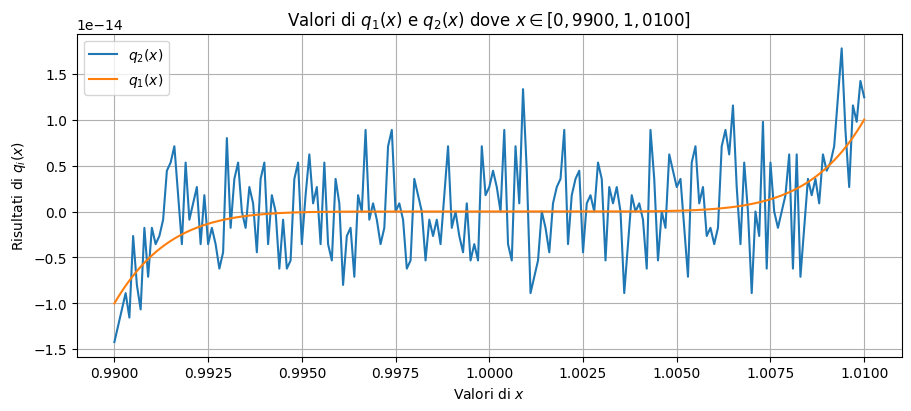
\includegraphics[width = \linewidth]{assets/image-001.png}
    \end{center}

    Notiamo infatti che, mentre $q_1(x)$ ha un comportamento più lineare, $q_2(x)$ è molto più scabro, e questo accade proprio a causa degli errori di approssimazione.
\end{example}

\section{La rappresentazione IEEE 754}

Ogni numero reale $x$ può essere espresso come una sequenza di infinite cifre, e tale sequenza dipende dalla \textbf{base di rappresentazione} $\beta$. Di norma, la base con cui noi esseri umani facciamo calcoli è $\beta = 10$.
\nwl
Qualsiasi cifra può essere espressa in qualsiasi base. Per farlo, faremo un esempio con $\pi$. Il numero infatti può essere scritto come segue:
\[ \pi \eq 3,14159... \eq \frac{3}{10^0} + \frac{1}{10^{-1}} + \frac{4}{10^{-2}} + \frac{1}{10^{-3}} + \frac{5}{10^{-4}} + \frac{9}{10^{-5}} + ... \]

L'idea è che per esprimere un qualsiasi numero $x$ in una base $\beta$, possiamo scrivere il numero come
\[ x \eq x_m \cdot \beta^m + x_{m-1} \cdot \beta^{m-1} + ... + x_{1} \cdot \beta^{1} + x_{0} \cdot \beta^{0} + x_{-1} \cdot \beta^{-1} + ... + x_{-m} \cdot \beta^{-m} \]

dove $0 \leq x_i \leq \beta - 1, \; \forall \; i \in [m, \; -m]$.
\nwl
Sappiamo che i computer funzionano in codice binario, quindi non possono interpretare i numeri in base decimale come facciamo noi umani. Per poter far sì che un computer riconosca un numero, questo va prima convertito in base 2. Ci sono vari modi per rappresentare un numero in binario: che sia con o senza segno, a virgola mobile o meno... C'è tuttavia uno standard che i computer adottano, che è stato sviluppato dall'IEEE, che viene usato per rappresentare tutti i numeri in binario, che abbiano un segno o che siano a virgola mobile: l'\textbf{IEEE 754}.
\nwl
Per questo standard, ogni numero può essere espresso nella seguente rappresentazione:
\[ x \eq \underbrace{\pm}_{\text{Segno}} \underbrace{(1 + a_{-1} \cdot 2^{-1} + a_{-2} \cdot 2^{-2} + a_{-3} \cdot 2^{-3} + ... + a_{-m} \cdot 2^{-m})}_{\text{Mantissa normalizzata}} \cdot \underbrace{2^e}_{\text{Esponente}} \]
\begin{center}
    \begin{tabular}{|c||c||c|}
        \hline
        $s$ & \hspace{1cm}$e$\hspace{1cm} & \hspace{3cm}$m$\hspace{3cm} \\
        \hline
    \end{tabular}
\end{center}

dove il segno viene rappresentato con 1 bit, la mantissa con $m$ bits e l'esponente con $n$ bits. Generalmente i numeri in IEEE 754 si possono esprimere con 16 (precisione dimezzata), 32 (singola precisione) o 64 bits (precisione doppia). Segue una tabella che segna quanti bits vengono assegnati ad ogni formato:
\begin{center}
    \begin{tabular}{|c|c|c|c|c|c|}
        \hline
        \textbf{Formato} & \textbf{Segno} & \textbf{Esponente} & \textbf{Mantissa} & \textbf{Bias} & \makecell{\textbf{Numero totale}\\\textbf{di bits}} \\
        \hline\hline
        \textbf{Precisione mezza} & 1 & 5 & 10 & 15 & 16 \\
        \hline
        \textbf{Singola precisione} & 1 & 8 & 23 & 127 & 32 \\
        \hline
        \textbf{Doppia precisione} & 1 & 11 & 52 & 1023 & 64 \\
        \hline
    \end{tabular}
\end{center}

Dato che i computer hanno una precisione finita, limitata a $p$ cifre, è chiaramente impossibile per questi rappresentare numeri che abbiano più di $p$ cifre. Per poter rappresentare numeri con più cifre, è necessario \textbf{arrotondare} il numero. L'arrotondamento può avvenire in due modi: o tramite \textbf{troncamento} o tramite \textbf{arrotondamento simmetrico}.

\begin{definition}{Troncamento e Arrotondamento simmetrico}
    Per \textbf{troncamento} si definisce quell'operazione per cui un numero a $n$ cifre viene rappresentato come un numero a $p$ cifre, dove le ultime $n - p$ cifre sono uguali a 0:
    \[ x^* \eq \text{tronc}(x) \thus x_{-k} \eq 0, \; \forall \; k \geq p \]

    Per \textbf{arrotondamento simmetrico} si definisce un'operazione di troncamento su un numero $x$ a cui può essere aggiunta un'unità alla cifra $x_{-p + 1}$ se la cifra $x_{-p}$ è maggiore o uguale di $\frac{\beta}{2}$:
    \[ x^* \eq \text{tronc}(x + 0,5 \cdot \beta^{-p+1} \cdot \beta^e) \thus \begin{cases}
        x_{-p + 1} = x_{-p + 1} & \text{se } x_{-p} < \frac{\beta}{2} \\
        x_{-p + 1} = x_{-p + 1} + 1 & \text{se } x_{-p} \geq \frac{\beta}{2}
    \end{cases}\]
\end{definition}

Arrotondare comporta sempre la presenza di un errore, e tali errori \textbf{non possono essere trascurati}, in quanto possono potenzialmente alterare il risultato finale in modi disastrosi. Un esempio è il caso del processore Intel Pentium (1994), che portava a risultati imperfetti a causa dell'arrotondamento dei numeri alla quinta cifra decimale.
\nwl
Un altro esempio di errore dato dall'arrotondamento è la \textbf{cancellazione numerica}. Per spiegare meglio questo fenomeno, consideriamo il seguente esempio:

\begin{example}
    Considerando un'equazione di secondo grado del tipo $ax^2 + bx + c = 0$, vogliamo calcolare le radici dell'equazione dati i valori di $a$, $b$ e $c$. Vogliamo calcolare $x_1$ e $x_2$ sia attraverso la formula classica delle radici (quindi $x \eq \frac{-b \pm \sqrt{\Delta}}{2a}$), sia attraverso una forma più compatta:
    \[ x_1 \eq \frac{2c}{-b + \sqrt{\Delta}} \quad\quad\quad x_2 \eq \frac{c}{ax_1} \]
    
    Per farlo, consideriamo il seguente script di Python, che con la funzione \verb|solve_f()| calcola le due radici con la formula classica e che con la funzione \verb|solve_f_alt()| calcola invece le due radici con le formule alternative sopra menzionate:

    \begin{codeblock}{NumericalAbsorption.py}
        \begin{lstlisting}[language = Python]
def solve_f(a, b, c) -> tuple[float, float]:
    delta = pow(b, 2) - 4 * a * c
    x1, x2 = (-b - sqrt(delta)) / (2 * a), (-b + sqrt(delta)) / (2 * a)
    return (x1, x2)

def solve_f_alt(a, b, c) -> tuple[float, float]:
    delta = pow(b, 2) - 4 * a * c
    x1 = (2 * c) / (-b + sqrt(delta))
    x2 = c / (a * x1)
    return (x1, x2)

def f(a, b, c, x) -> float:
    return a * pow(x, 2) + b * x + c


inputs = [[1, 4, 3], [1, -206.5, 0.01021]]
for a, b, c in inputs:
    x1, x2 = solve_f(a, b, c)
    print(f"With a = {a}, b = {b}, c = {c}\n  x1 = {x1}\n  x2 = {x2}\n  f({x1}) = {f(a, b, c, x1)}\n  f({x2}) = {f(a, b, c, x2)}\n")

    x1, x2 = solve_f_alt(a, b, c)
    print(f"Second method\n  x1 = {x1}\n  x2 = {x2}\n  f({x1}) = {f(a, b, c, x1)}\n  f({x2}) = {f(a, b, c, x2)}\n\n")\end{lstlisting}
    \end{codeblock}

    Raccogliamo gli output della prima parte del codice nella seguente tabella, in cui mostriamo i risultati ottenuti con la funzione \verb|solve_f()|:

    \begin{center}
        \begin{tabular}{|c|c|c|c|c|}
            \hline
            $\mathbf{a,\; b,\; c}$ & $\mathbf{x_1}$ & $\mathbf{x_2}$ & $\mathbf{f(x_1)}$ & $\mathbf{f(x_2)}$ \\
            \hline\hline
            $1, \; 3, \; 4$ & $-3$ & $-1$ & $0$ & $0$ \\
            \hline
            \makecell{$1, \; -206,5,$\\$0,01021$} & \makecell{$4,944... \cdot 10^{-5}$} & $206,499...$ & $5,454... \cdot 10^{-13}$ & $-3,702... \cdot 10^{-13}$ \\
            \hline
        \end{tabular}
    \end{center}

    In questa seconda tabella invece, raccogliamo i risultati ottenuti grazie alla funzione \verb|solve_f_alt()|:

    \begin{center}
        \begin{tabular}{|c|c|c|c|c|}
            \hline
            $\mathbf{a,\; b,\; c}$ & $\mathbf{x_1}$ & $\mathbf{x_2}$ & $\mathbf{f(x_1)}$ & $\mathbf{f(x_2)}$ \\
            \hline\hline
            $1, \; 3, \; 4$ & $-3$ & $-1$ & $0$ & $0$ \\
            \hline
            \makecell{$1, \; -206,5,$\\$0,01021$} & \makecell{$4,944... \cdot 10^{-5}$} & $206,499...$ & $1,734... \cdot 10^{-18} \simeq 0_m$ & $-3,702... \cdot 10^{-13}$ \\
            \hline
        \end{tabular}
    \end{center}

    Sebbene per il primo set di inputs (quindi con $a \eq 1$, $b \eq 3$ e $c \eq 4$) i risultati siano gli stessi, con il secondo set i risultati iniziano ad essere diversi da quel che ci aspetteremmo. Infatti, il risultato di $f(x_1)$ e $f(x_2)$ dovrebbe essere uguale a 0, eppure è sempre un numero abbastanza vicino allo zero (nella seconda tabella, il risultato di $f(x_1)$ per il secondo set di inputs è infatti segnato come simile allo zero macchina, $0_m$).
    \nwl
    Ancora più interessante è il risultato di $x_1$, quando viene usato il secondo set di inputs: il valore infatti è dato da $-b - \sqrt{\Delta}$, che, dati i nostri inputs, corrisponde al calcolo della differenza tra $b$ e $\sqrt{\Delta}$. Questi due numeri però sono molto vicini fra di loro, e la loro differenza è un esempio di cancellazione numerica.
    \nwl
    Realmente, la loro differenza dovrebbe risultare in un numero infinitesimamente piccolo, ma il computer lo approssima a $0$ per impossibilità di immagazzinare numeri infinitesimamente piccoli.
\end{example}

Un errore non è mai fine a sé stesso: è possibile (talvolta certo) che si propaghi e che influenzi i risultati delle operazioni future. Definiamo qui i vari tipi di errori che si creano in base all'operazione che viene performata:
\begin{definition}{Errori di propagazione}
    Si consideri come $fl(n)$ la rappresentazione in virgola mobile arrotondata del numero $n$, e si denoti con $e_n$ l'errore corrispondente, cosicché:
    \[ e_n \eq \frac{fl(n) - n}{n} \thus fl(n) \eq n \cdot e_n + n \eq x \cdot (1 + e_n) \]

    Si considerino due numeri $x$ e $y$, e le loro rispettive rappresentazioni in virgola mobile. Definiamo i seguenti errori:
    \begin{itemize}
        \item \textbf{errore del prodotto} $e_{xy}$:
        \[ fl(x) \cdot fl(y) \eq (x \cdot (1 + e_x)) \cdot (y \cdot (1 + e_y)) \eq xy \cdot (1 + \underbrace{e_x + e_y}_{e_{xy}} + e_x \cdot e_y) \; \simeq \; xy \cdot (1 + \underbrace{e_x + e_y}_{e_{xy}}) \]

        \item \textbf{errore della divisione} $e_{\frac{x}{y}}$:
        \[ \frac{fl(x)}{fl(y)} \eq \frac{x \cdot (1 + e_x)}{y \cdot (1 + e_y)} \eq \frac{x}{y} \cdot (1 + e_x) \cdot (1 - e_y + e^2_y + ...) \; \simeq \; \frac{x}{y} \cdot (1 + \underbrace{e_x - e_y}_{e_{\frac{x}{y}}}) \]

        \item \textbf{errore della somma} $e_{x+y}$:
        \[ fl(x) + fl(y) \eq x \cdot(1 + e_x) + y \cdot (1 + e_y) \simeq x + y + xe_x + ye_y \eq \]
        \[ \eq (x + y) \cdot \left(1 + \underbrace{\frac{x}{x + y} \cdot e_x + \frac{y}{x + y} \cdot e_y}_{e_{x+y}} \right) \]

        In quest'ultimo caso, se $x, y > 0$, allora $|e_{x+y}| \leq |e_x| + |e_y|$; se $x, y < 0$, allora le quantità $\left|\frac{x}{x + y}\right|$ e $\left|\frac{y}{x + y}\right|$ possono essere molto grandi
    \end{itemize}
\end{definition}

\section{Algoritmi e Condizionamento dei problemi}

Fin dall'antica Grecia c'è sempre stata varia ambiguità su cosa fosse un algoritmo e su come definirlo, nonostante ci fosse sempre stata un'intuizione. È solo grazie alla tesi di Church-Turing nel 1936, che fu possibile definire formalmente cosa fosse un algoritmo (definito nella tesi come \textit{metodo efficace}):

\begin{quotebox}{Church-Turing}
    "Un metodo efficace è un metodo per cui ogni istruzione è precisamente pre-determinata, che è certo di produrre un output entro un numero finito di istruzioni"
\end{quotebox}

Possiamo tuttavia riformulare la tesi di Church-Turing per definire cosa sia un algoritmo, così da adattarla anche per i nostri scopi:

\begin{definition}{Algoritmo}
    Un \textbf{algoritmo} è una successione di \textbf{istruzioni} \textbf{finita} e \textbf{non ambigua}, che consente di ottenere risultati numerici a partire dai dati di input
\end{definition}

Gli algoritmi che formuleremo attraverso queste note verranno implementate su un computer tramite un linguaggio di programmazione. Tutte le istruzioni sono operazioni logiche o aritmetiche, che vengono assegnate al computer seguendo la sintassi del linguaggio che useremo.
\nwl
Come abbiamo visto in precedenza, la propagazione di un errore può avere effetti disastrosi, anche se l'errore è molto "piccolo". Se l'errore dovesse amplificarsi ad alti livelli, il risultato ottenuto non sarebbe affidabile. In questo caso, diremmo che l'algorimo è \textbf{instabile}. Se invece gli errori di arrotondamento non vengono amplificati durante i calcoli, allora diciamo che l'algoritmo è \textbf{stabile}.

\begin{example}
    Data la funzione $f(x) = x^2 + 2px - q$, con $p^2 + q \geq 0$, vogliamo calcolare la radice di valore maggiore. Questa è data dalla seguente equazione
    \[ y = -p + \sqrt{p^2 + q} \]

    Proviamo a creare uno script di Python che esegua questa equazione e che calcoli anche l'errore tra la soluzione del computer e quella prevista (usando la funzione \verb|rounding_error()| dall'esempio 1.1.1)

    \begin{codeblock}{AlgorithmStability-Part1.py}
        \begin{lstlisting}[language = Python]
P = 1000
Q = 0.018000000081
SOLUTION = 0.9 * pow(10, -5)

def solve_r1(p, q) -> float:
    return -p + sqrt(pow(p, 2) + q)

r1 = solve_r1(P, Q)

print(f"[Algorithm 1] y = {r1}\n[Algorithm 1] Error = {rounding_error(SOLUTION, r1)}")\end{lstlisting}
        \nwl
        \begin{tcolorbox}[colback = black!95!Periwinkle!90]
            \begin{lstlisting}[style = notexterm]
Out[1]: [Algorithm 1] y = 8.999999977277184e-06
        [Algorithm 1] Error = 2.2722815857102556e-14\end{lstlisting}
        \end{tcolorbox}
    \end{codeblock}

    Come possiamo notare, l'errore è abbastanza cospicuo, e per questo l'algoritmo è detto instabile. Questo perché, per $p \gg q$, la sottrazione tra $p$ e $\sqrt{p^2 + q}$ comporta la cancellazione numerica. Proviamo invece con un altro algoritmo, che cerca di arrivare allo stesso risultato senza usare la sottrazione, così da essere stabile:

    \[ y = -p + \sqrt{p^2 + q} \eq \left(-p + \sqrt{p^2 + q}\right) \cdot \frac{\left(p + \sqrt{p^2 + q}\right)}{\left(p + \sqrt{p^2 + q}\right)} \eq \frac{q}{\left(p + \sqrt{p^2 + q}\right)} \]

    \begin{codeblock}{AlgorithmStability-Part2.py}
        \begin{lstlisting}[language = Python]
def solve_r2(p, q) -> float:
    return q / (p + sqrt(pow(p, 2) + q))

r2 = solve_r2(P, Q)

print(f"[Algorithm 2] y = {r2}\n[Algorithm 2] Error = {rounding_error(SOLUTION, r2)}")\end{lstlisting}
        \nwl
        \begin{tcolorbox}[colback = black!95!Periwinkle!90]
            \begin{lstlisting}[style = notexterm]
Out[1]: [Algorithm 2] y = 9e-06
        [Algorithm 2] Error = 0.0\end{lstlisting}
        \end{tcolorbox}
    \end{codeblock}
\end{example}

Non solo gli algoritmi possono essere stabili o instabili, ma in base a come vengono posti i problemi ci può essere più o meno suscettibilità alle perturbazioni dei dati. Consideriamo ad esempio il seguente problema: abbiamo una funzione $f \; : \; \mathbb{R} \; \mapsto \; \mathbb{R}$, e vogliamo calcolarne il valore $y$ in un generico punto $x \in \mathbb{R}$. Normalmente avremmo che $x \; \rightarrow \; f(x) \; \rightarrow \; y$.
\nwl
Ottenuto $y$, vogliamo misurare quale effetto produca una perturbazione $\Delta x = x^* - x$ (dove $x^*$ è un valore a nostra scelta) durante il calcolo di $y$. Possiamo inoltre riconsiderare $\Delta x$ come il seguente: $\Delta y \eq y^* - y = f(x^*) - f(x)$
\nwl
Usando lo sviluppo in serie di Taylor fino al primo ordine, possiamo riscrivere $\Delta y$ come segue:
\[ \Delta y \eq f(x^*) - f(x) \eq f'(x) \cdot \underbrace{\Delta x}_{x^* - x} \]

Dividendo ciò che abbiamo ottenuto fino ad ora per $y$, possiamo ricavare l'\textbf{errore relativo}:
\[ \left| \frac{\Delta y}{y} \right| \; \simeq \; \left| \frac{f'(x)}{f(x)} \right| \cdot \left|\Delta x\right| \eq \underbrace{\left| \frac{f'(x) \cdot x}{f(x)} \right|}_{C_P} \cdot \left|\frac{\Delta x}{x}\right| \]

\begin{definition}{Errore relativo}
    L'\textbf{errore relativo} $e_r$ è l'errore che c'è tra un valore $x^*$ e un valore comparato $x$, ed è sempre \textbf{espresso in percentuale}. Tale errore si calcola come segue:
    \[ e_r \eq \frac{\left| x^* - x \right|}{x} \]
\end{definition}

Nel calcolo precedente abbiamo evidenziato una parte dell'equazione, chiamandola $C_P$. Tale numero è importante per noi, e si chiama \textbf{numero di condizionamento del problema}.

\begin{definition}{Numero di condizionamento del problema}
    Il \textbf{numero di condizionamento del problema} $C_P$ è un numero che determina se un dato problema è \textbf{malcondizionato} (ovverosia che a \textbf{piccole perturbazioni} dei dati corrispondono \textbf{grandi variazioni} dei risultati) o \textbf{ben condizionato}. Se $C_P$ è \textbf{grande}, allora il problema è \textbf{malcondizionato}, altrimenti è ben condizionato.
    \[ C_P \eq \left| \frac{f'(x) \cdot x}{f(x)} \right| \]
\end{definition}

Sebbene la propagazione dell'errore dipenda dall'algoritmo, il condizionamento del problema non dipende né dall'algoritmo, né dagli errori generati. Infatti, il \textbf{condizionamento dipende solo ed unicamente dal problema} e dai dati di input. Se il problema è molto sensibile, e quindi malcondizionato, alle variazioni di input, allora \textbf{non esiste nessun algoritmo} che riesca a ritornare una soluzione stabile al problema.
    \pagebreak
    \chapter{MATLAB}

MATLAB è un linguaggio di programmazione sviluppato negli anni '70, che viene usato per sviluppare modelli matematici, svolgere simulazioni e analisi dei dati. Il modo in cui MATLAB funziona è detto \textbf{interattivo}, poiché viene tutto eseguito nella console. È possibile anche eseguire più comandi assieme nello stesso prompt, separando tutti i comandi con delle virgole. Ad esempio:

\begin{terminal}
    \begin{lstlisting}[language=MATLAB, style=notexterm]
>> 2+3, 7*2, 9+1*3\end{lstlisting}
    \tcblower
    \begin{lstlisting}[style=notexterm]
ans = 5
ans = 14
ans = 12\end{lstlisting}
\end{terminal}

Operazioni più lunghe possono essere scritte su più righe usando i "\texttt{...}". Gli operatori disponibili sono i seguenti:

\begin{center}
    \begin{tabular}{|c|c|}
        \hline
        \textbf{Operazione} & \textbf{Operatore} \\
        \hline \hline
        Somma & \texttt{+} \\
        \hline
        Sottrazione & \texttt{-} \\
        \hline
        Moltiplicazione & \texttt{*} \\
        \hline
        Divisione & \texttt{/} \\
        \hline
        Potenza & \verb|^| \\
        \hline\hline
        Minore & \texttt{<} \\
        \hline
        Maggiore & \texttt{>} \\
        \hline
        Minore o uguale & \texttt{<=} \\
        \hline
        Maggiore o uguale & \texttt{>=} \\
        \hline
        Uguale & \texttt{==} \\
        \hline
        Diverso & \verb|~=| \\
        \hline
    \end{tabular}
\end{center}

In MATLAB, è possibile anche usare gli operatori logici, quali l'\texttt{AND}, l'\texttt{OR} e il \texttt{NOT}. Chiaramente, anche i gate logici più complessi, che vengono costruiti con gli operatori logici più semplici, sono disponibili.

\begin{center}
    \begin{tabular}{|c|c|}
        \hline
        \textbf{Operazione} & \textbf{Operatore} \\
        \hline \hline
        \texttt{AND} & \verb|&| \\
        \hline
        \texttt{OR} & \texttt{|} \\
        \hline
        \texttt{NOT} & \verb|~| \\
        \hline
    \end{tabular}
\end{center}

Ci sono anche alcune costanti, che vengono incluse in MATLAB di default dalla libreria standard. Qui alcune di queste vengono elencate:

\begin{center}
    \begin{tabular}{|c|c|}
        \hline
        \textbf{Operazione} & \textbf{Operatore} \\
        \hline\hline
        Infinito ($\infty$) & \texttt{inf} \\
        \hline
        $\pi$ & \texttt{pi} \\
        \hline
        $i$ & \texttt{i} \\
        \hline
        Numero massimo rappresentabile & \texttt{realmax} \\
        \hline
        Numero minimo rappresentabile & \texttt{realmin} \\
        \hline
        Precisione della macchina & \texttt{eps} \\
        \hline
        Forma indeterminata / \texttt{Not A Number} & \texttt{nan} \\
        \hline
    \end{tabular}
\end{center}

Nella scorsa tabella, i valori \texttt{realmax} e \texttt{realmin} si riferiscono rispettivamente al valore massimo e minimo rappresentabile considerando numeri in IEEE 754 a doppia precisione (dunque a 64 bits). La libreria standard di MATLAB possiede varie funzioni matematiche, tra cui $\sin (x)$, $\cos (x)$, $\tan (x)$, $\log (x)$, etc... Nel caso in cui si volessero avere più informazioni circa una funzione, si può usare la funzione \texttt{help <funzione>}, dove \texttt{<funzione>} è la funzione di cui vogliamo ottenere più informazioni. Ad esempio:

\begin{terminal}
    \begin{lstlisting}[language=MATLAB, style=notexterm]
>> help log\end{lstlisting}
    \tcblower
    \begin{lstlisting}[style=notexterm, language = tex]
 log - Natural logarithm
    This MATLAB function returns the natural logarithm ln(x) of each element
    in array X.

    Syntax
        Y = log(X)

    Input Arguments
        X - Input array
        scalar | vector | matrix | multidimensional array | table |
        timetable

    Output Arguments
        Y - Logarithm values
        scalar | vector | matrix | multidimensional array | table |
        timetable

    Examples
        Natural Logarithm of Negative Number

    See also log1p, log2, log10, exp, logm, reallog, loglog, semilogx,
        semilogy

    Introduced in MATLAB before R2006a
    Documentation for log
    Other uses of log\end{lstlisting}
\end{terminal}

Se dovessimo aver bisogno di una funzione che svolga un certo compito, ma non ci dovessimo ricordare qual'è la funzione adatta, possiamo usare invece la funzione \texttt{lookfor <keywords>}, dove \texttt{<keywords>} è un insieme di keywords per identificare la funzione che cerchiamo. Ad esempio:

\begin{terminal}
    \begin{lstlisting}[language=MATLAB, style=notexterm]
>> lookfor square\end{lstlisting}
    \tcblower
    \begin{lstlisting}[style=notexterm, language = tex]
cgs                            - Solve system of linear equations - conjugate
                                 gradients squared method
deconv                         - Least-squares deconvolution and polynomial 
                                 division
hypot                          - Square root of sum of squares (hypotenuse)
lscov                          - Least-squares solution in presence of known 
                                 covariance
lsqminnorm                     - Minimum norm least-squares solution to 
                                 linear equation
lsqnonneg                      - Solve nonnegative linear least-squares 
                                 problem
lsqr                           - Solve system of linear equations - 
                                 least-squares method
[...]\end{lstlisting}
\end{terminal}

\section{Variabili, handling della memoria e formati}

Le variabili su MATLAB vengono assegnate e dichiarate similmente a Python: l'assegnazione e la dichiarazione avvengono allo stesso momento. Ad esempio, se volessimo dichiarare la variabile $a=4$ ci basterebbe eseguire il seguente codice:

\begin{terminal}
    \begin{lstlisting}[language=MATLAB, style=notexterm]
>> a = 4\end{lstlisting}
    \tcblower
    \begin{lstlisting}[style=notexterm, language = tex]
a = 4\end{lstlisting}
\end{terminal}

Possiamo visualizzare il contenuto di una variabile in due modi: o chiamando la variabile nella console, o usando la funzione \texttt{disp(<variabile>)}. Segue un esempio:

\begin{terminal}
    \begin{lstlisting}[language=MATLAB, style=notexterm]
>> a
>> disp(a)\end{lstlisting}
    \tcblower
    \begin{lstlisting}[style=notexterm, language = tex]
a = 4

4\end{lstlisting}
\end{terminal}

Per cancellare tutte le variabili dalla memoria si usa il comando \texttt{clear}. Per salvarne alcune tra una sessione e l'altra, possiamo usare il comando \texttt{save <filename> [<var1> <var2> ...]}, dove \texttt{<filename>} è il file in cui salveremo le variabili (in estensione \texttt{.mat}), mentre \texttt{[<var1> <var2> ...]} è una lista di variabili che vogliamo salvare. Ad esempio:

\begin{terminal}
    \begin{lstlisting}[language=MATLAB, style=notexterm]
>> b = 5;
>> c = 7;
>> save Vars/someVars b c\end{lstlisting}
\end{terminal}

Una volta cancellate le variabili dalla memoria, usando il comando \texttt{who} non le vedremmo più. Possiamo caricare nuovamente le variabili all'interno di MATLAB usando il comando \texttt{load <filename>}, che caricherà tutte le variabili all'interno del file \texttt{<filename>}. Non è necessario includere l'estensione \texttt{.mat}.

\begin{terminal}
    \begin{lstlisting}[language=MATLAB, style=notexterm]
>> load Vars/someVars
>> who\end{lstlisting}
    \tcblower
    \begin{lstlisting}[style=notexterm, language = tex]
Your variables are:

b  c  \end{lstlisting}
\end{terminal}

MATLAB ha vari formati per i dati, simili concettualmente ai tipi di Python, molto vicini ai tipi di C. Ad esempio:

\begin{center}
    \begin{tabular}{|c|c|}
        \hline
        \textbf{Formato} & \textbf{Descrizione} \\
        \hline\hline
        \texttt{double} & Numeri in doppia precisione \\
        \hline
        \texttt{uint8} & Interi senza segno a 8 bits \\
        \hline
        \texttt{uint16} & Interi senza segno a 16 bits \\
        \hline
        \texttt{uint32} & Interi senza segno a 32 bits \\
        \hline
        \texttt{int8} & Interi con segno a 8 bits \\
        \hline
        \texttt{int16} & Interi con segno a 16 bits \\
        \hline
        \texttt{int32} & Interi con segno a 32 bits \\
        \hline
        \texttt{single} & Numeri a singola precisione \\
        \hline
        \texttt{char} & Caratteri, 2 bytes per carattere \\
        \hline
        \texttt{logical} & Valore che è o \texttt{0} o \texttt{1}, generalmente usato come valore Booleano \\
        \hline
    \end{tabular}
\end{center}

Possiamo impostare anche un formato di visualizzazione dei dati tramite la funzione \texttt{format}. Tuttavia, questo formato sarà valido \textbf{solo per la visualizzazione dei dati}: all'interno di MATLAB i calcoli verranno effettuati con la stessa precisione standard di MATLAB. Facciamo un esempio:

\begin{terminal}
    \begin{lstlisting}[language=MATLAB, style=notexterm]
>> % Qui MATLAB mostrerà i dati in formato short
   sqrt(2)

>> % Con long aumentiamo il formato
   format long
   sqrt(2)\end{lstlisting}
    \tcblower
    \begin{lstlisting}[style=notexterm, language = tex]
ans = 1.4142

ans = 
   1.414213562373095\end{lstlisting}
\end{terminal}

Se volessimo cambiare il tipo dei dati, possiamo farlo usando i costruttori dei vari tipi. Ad esempio:

\begin{terminal}
    \begin{lstlisting}[language=MATLAB, style=notexterm]
>> a = 43.97;

>> int16(a)
>> double(a)
>> uint8(a)\end{lstlisting}
    \tcblower
    \begin{lstlisting}[style=notexterm, language = tex]
ans = int1644

ans = 43.9700

ans = uint844\end{lstlisting}
\end{terminal}

\section{Tipi di dati}

Oltre ai formati di numeri menzionati fino ad ora, MATLAB ha anche altri tipi di dati, che ritornano comodi per esprimere costrutti matematici come vettori, matrici e tabelle.

\subsection{Vettori, matrici e tensori}

In MATLAB è possibile usare vettori, matrici e in generale tensori a $n$ dimensioni. Come in C e in Python, vettori e matrici sono realizzabili tramite array a rispettivamente una e due dimensioni. Anche le variabili in realtà sono considerate internamente come arrays: infatti uno scalare è rappresentato tramite matrici a dimensione $1\times 1$. Possiamo realizzare vettori riga e vettori colonna, in base al carattere usato per separare i valori:
\begin{itemize}
    \item usando la virgola \texttt{,} (o degli spazi) possiamo creare vettori riga;
    \item usando il punto e virgola \texttt{;} possiamo creare vettori colonna.
\end{itemize}

\begin{terminal}
    \begin{lstlisting}[language=MATLAB, style=notexterm]
>> A = [10, 20, 30, 40, 50]
>> B = [10; 20; 30; 40; 50]\end{lstlisting}
    \tcblower
    \begin{lstlisting}[style=notexterm, language = tex]
A = 1x5
    10    20    30    40    50

B = 5x1
    10
    20
    30
    40
    50\end{lstlisting}
\end{terminal}

Per ottenere il trasposto di un vettore o di una matrice, si usa il simbolo \texttt{'}:

\begin{terminal}
    \begin{lstlisting}[language=MATLAB, style=notexterm]
>> A'\end{lstlisting}
    \tcblower
    \begin{lstlisting}[style=notexterm, language = tex]
ans = 5x1
    10
    20
    30
    40
    50\end{lstlisting}
\end{terminal}

Per ottenere invece il valore posto in una certa posizione di un vettore, si usa la seguente notazione: \texttt{vettore(posizione)}. In MATLAB, \textbf{gli indici non partono da 0, ma da 1}. Possiamo usare anche una notazione simile allo slicing di Python. Infatti, esiste una notazione più complessa, che è \texttt{vettore(inizio:passo:fine)}, dove \texttt{inizio} determina l'indice di inizio della sequenza che vogliamo esprimere, \texttt{passo} indica ogni quanti elementi serve prendere un valore, \texttt{fine} (\textbf{inclusivo}) indica quando fermarsi con lo slice. Ad esempio:

\begin{terminal}
    \begin{lstlisting}[language=MATLAB, style=notexterm]
>> A(1:2:4)\end{lstlisting}
    \tcblower
    \begin{lstlisting}[style=notexterm, language = tex]
ans = 1x2
    10    30\end{lstlisting}
\end{terminal}

Con questa notazione possiamo anche creare nuovi vettori. Ad esempio:

\begin{terminal}
    \begin{lstlisting}[language=MATLAB, style=notexterm]
>> C = [0.9:0.01:1.1]\end{lstlisting}
    \tcblower
    \begin{lstlisting}[style=notexterm, language = tex]
C = 1x21
    0.9000    0.9100    0.9200    0.9300    0.9400    0.9500    0.9600    0.9700    0.9800    0.9900    1.0000    1.0100    1.0200    1.0300    1.0400    1.0500    1.0600    1.0700    1.0800    1.0900    1.1000\end{lstlisting}
\end{terminal}

Contrariamente a C, la dimensione e i valori di un array possono essere modificati in corso d'opera. Ad esempio, avendo un array di 4 elementi, possiamo modificare il 6° elemento dell'array, accedendovi come se esistesse:

\begin{terminal}
    \begin{lstlisting}[language=MATLAB, style=notexterm]
>> D = [1:2:7]
>> D(6) = 11\end{lstlisting}
    \tcblower
    \begin{lstlisting}[style=notexterm, language = tex]
D = 1x4
    1     3     5     7

D = 1x6
    1     3     5     7     0    11\end{lstlisting}
\end{terminal}

Alle posizioni non definite, come possiamo notare, viene assegnato il valore 0.
\nwl
Un'operazione particolare, soprattutto quando si usano i vettori (vedi dopo) è l'evelamento a potenza. Normalmente l'elevamento a potenza viene fatto con la notazione \texttt{\textasciicircum n}, tuttavia esiste una seconda notazione: la notazione \texttt{.\textasciicircum n} indica che viene fatta la potenza alla $n$ di ogni singola componente di un vettore. Senza il . allora verrebbe fatto l'elevamento a potenza di un vettore moltiplicando il vettore per se stesso. Ad esempio:

\begin{terminal}
    \begin{lstlisting}[language=MATLAB, style=notexterm]
>> D = [3, 7; 14, 21];
>> D^2
>> D.^2\end{lstlisting}
    \tcblower
    \begin{lstlisting}[style=notexterm, language = tex]
ans = 2x2
    107   168
    336   539

ans = 2x2
      9    49
    196   441\end{lstlisting}
\end{terminal}

\subsection{Celle}

Un'ultima struttura dati che è molto comoda è la cell. Una cell è un array di valori dinamico, dove i valori possono avere tipi diversi. Una cell si definisce in questo modo:

\begin{terminal}
    \begin{lstlisting}[language=MATLAB, style=notexterm]
>> C = {"Hello world", [4, 6, 8], 16, -92.77, [16, 32, 11; 4, 97, 6; 14, 9, 8]}\end{lstlisting}
    \tcblower
    {
        \color{white} \ttfamily
        \begin{tabular} {|c|c|c|c|c|c|}
        \hline
         & 1 & 2 & 3 & 4 & 5 \\
        \hline
        1 & "Hello world" & [4,6,8] & 16 & -92.7700 & [16,32,11;4,97,6;14,9,8] \\ 
        \hline
        \end{tabular}
    }
\end{terminal}

Possiamo controllare il valore all'interno di un elemento di una cella con la notazione \texttt{cella(indice)}:

\begin{terminal}
    \begin{lstlisting}[language=MATLAB, style=notexterm]
>> C(1)\end{lstlisting}
    \tcblower
    \begin{lstlisting}[style=notexterm, language = tex]
ans = 1x1 cell array
    {["Hello world"]}\end{lstlisting}
\end{terminal}

Possiamo anche estrarre un elemento da una cella tramite la notazione \texttt{cella\{indice\}}:

\begin{terminal}
    \begin{lstlisting}[language=MATLAB, style=notexterm]
>> A = C{1}\end{lstlisting}
    \tcblower
    \begin{lstlisting}[style=notexterm, language = tex]
A = "Hello world"\end{lstlisting}
\end{terminal}

Una cell non contiene i puntatori alle variabili inserite all'interno di essa, ma contiene delle copie identiche dei dati. Questo vuol dire che se una certa variabile viene inserita dentro la cell, se si modificasse la variabile allora il valore nella cell non si aggiornerebbe. I valori in una cell possono essere modificati usando la seguente notazione:

\begin{terminal}
    \begin{lstlisting}[language=MATLAB, style=notexterm]
>> C(1) = {"Ciao mondo"}\end{lstlisting}
    \tcblower
    {
        \color{white} \ttfamily
        \begin{tabular} {|c|c|c|c|c|c|}
        \hline
         & 1 & 2 & 3 & 4 & 5 \\
        \hline
        1 & "Ciao mondo" & [4,6,8] & 16 & -92.7700 & [16,32,11;4,97,6;14,9,8] \\ 
        \hline
        \end{tabular}
    }
\end{terminal}

\subsection{Structs}

Una struct in MATLAB è simile a una struct in C: questa ha dei campi nominali che possono essere modificati a piacimento. Ad esempio:

\begin{terminal}
    \begin{lstlisting}[language=MATLAB, style=notexterm]
>> S.string = "Hello world"
>> S.value = 32
>> S.matrix = [2, 4; 5, 7]\end{lstlisting}
    \tcblower
    \begin{lstlisting}[style=notexterm, language = tex]
S = struct with fields:
    string: "Hello world"

S = struct with fields:
    string: "Hello world"
     value: 32
    
S = struct with fields:
    string: "Hello world"
    value: 32
    matrix: [2x2 double]\end{lstlisting}
\end{terminal}

Possiamo estrarre i valori all'interno di un campo chiamando il campo stesso:

\begin{terminal}
    \begin{lstlisting}[language=MATLAB, style=notexterm]
>> S.value\end{lstlisting}
    \tcblower
    \begin{lstlisting}[style=notexterm, language = tex]
ans = 32\end{lstlisting}
\end{terminal}

\section{Funzioni}

Come molti linguaggi di programmazione, MATLAB consente lo sviluppo di funzioni definite dall'utente, e questo si fa tramite la seguente notazione:

\begin{verbatim}
  function [output1, output2, ...] = nome_funzione(input1, input2, ...)
      % Codice...
  end
\end{verbatim}

Segue un esempio di una funzione che calcola il $\Delta$ di un'equazione di secondo grado:

\begin{terminal}
    \begin{lstlisting}[language=MATLAB, style=notexterm]
function [out] = custom_delta(a, b, c)
% Calcola il delta di una data equazione di secondo grado, dati i coefficienti
% a, b e c
    out = b^2 - 4*a*c;
end\end{lstlisting}
\end{terminal}

Possiamo testarne il funzionamento chiamando la funzione stessa, considerando ad esempio la funzione $4x^2 + 11x - 3 \eq 0$:

\begin{terminal}
    \begin{lstlisting}[language=MATLAB, style=notexterm]
>> [d1] = custom_delta(4, 11, -3)\end{lstlisting}
    \tcblower
    \begin{lstlisting}[style=notexterm, language = tex]
d1 = 169\end{lstlisting}
\end{terminal}

\subsection{Funzioni particolari}

Alcune funzioni particolari di MATLAB, che potrebbero risultare utili, sono le seguenti:
\begin{itemize}
    \item \texttt{diff(x)}: dato un vettore $x$ di $n$ elementi, \texttt{diff(x)} calcola un vettore di $n - 1$ elementi dove ogni elemento $y_i$ è uguale alla seguente operazione: $y_i \eq -x_i + x_{i + 1}$. Tale funzione può anche avere un parametro extra, l'ordine. Questo parametro indica che \texttt{diff(x)} viene chiamato ricorsivamente tante volte quanto specifica l'ordine. Con le matrici, la differenza viene fatta considerando le righe della matrice. Partendo da una matrice $A$ di dimensioni $m \times n$, la matrice finale avrà come dimensioni $(m - 1)\times n$. Ad esempio: 
    \begin{terminal}
        \begin{lstlisting}[language=MATLAB, style=notexterm]
>> A = [-2, 5, -3, 6, -1, 4];
>> B = [4, 7, 8; 11, 4, -3; 16, 7, 9];

>> % Diff(A) con ordine 1
>> diff(A)

>> % Diff(A) con ordine 2
>> diff(A, 2)

>> % Diff(B) con ordine 1
>> diff(B)\end{lstlisting}
        \tcblower
        \begin{lstlisting}[style=notexterm, language = tex]
ans = 1x5
    7    -8     9    -7     5

ans = 1x4
    -15    17   -16    12

ans = 2x3
    7    -3   -11
    5     3    12\end{lstlisting}
    \end{terminal}
    \item \texttt{find(cond)}: data una condizione, \texttt{find()} ritorna tutti gli indici in un vettore che rispettano la condizione. Ad esempio:
    \begin{terminal}
        \begin{lstlisting}[language=MATLAB, style=notexterm]
>> A = [3, 0.4, -16, 7, 11, -2, 9.07, 8];
>> x = find(mod(A, 2) == 0)\end{lstlisting}
        \tcblower
        \begin{lstlisting}[style=notexterm, language = tex]
x = 1x3
    3     6     8\end{lstlisting}
    \end{terminal}
\end{itemize}

\section{Costrutti di flow control}

Ci sono vari costrutti di flow control presenti in MATLAB, quali il \texttt{for} loop, il \texttt{while} loop e il condizionale \texttt{if - else if - else}.
    \pagebreak
    \chapter{Sistemi di Equazioni Non Lineari}

Fino ad ora siamo sempre stati abituati a problemi analitici dove la soluzione a un problema era data da un'equazione, o al più un piccolo sistema di equazioni non lineari. Tuttavia nella realtà sono molti i casi dove la soluzione viene trovata risolvendo complessi sistemi di equazioni non lineari, che non sempre possono essere svolti a mano. Da qui, la nascita di alcuni metodi di calcolo numerico che aiutano nella risoluzione di tali sistemi. Prima di illustrare questi metodi, ci soffermeremo brevemente su cos'è un'equazione non lineare:

\begin{definition}{Equazione non lineare}
    Un'\textbf{equazione non lineare} è un'equazione avente la forma
    \[ f(x) \eq 0 \]

    Chiamamo \textbf{soluzione} $\xi$ (o alternativamente \textbf{radici dell'equazione} o \textbf{zeri della funzione} $f$) di un'equazione non lineare quel valore tale che
    \[ f(\xi) \eq 0 \]
\end{definition}

All'interno di questo capitolo ci limiteremo prevalentemente al caso di radici reali. Per applicare un metodo su una funzione tuttavia, ci serve prima sapere le seguenti tre informazioni:
\begin{itemize}
    \item [1)] \textbf{quante} sono le radici (in questo caso, reali);
    \item [2)] \textbf{dove} si trovano, approssimativamente, le radici;
    \item [3)] se sono presenti delle \textbf{simmetrie} nella funzione.
\end{itemize}

Ci sono vari metodi per trovare queste informazioni: si può procedere allo \textbf{studio analitico}, alla \textbf{tabulazione} o all'analisi del \textbf{grafico} della funzione stessa. Procederemo ad illustrare tutti e tre i metodi su un'equazione di esempio:

\begin{example}
    Si consideri la seguente funzione $f(\lambda)$, che modella il tasso di crescita di una popolazione:
    \[ f(\lambda) \eq e^{\lambda} + \frac{0,435}{\lambda} (e^{\lambda} - 1) - 1,564 \eq 0 \]

    Procediamo a considerare lo \textbf{studio analitico} di questa funzione: notiamo che la funzione risulta definita e continua in $\mathbb{R} / \{0\}$, e studiando il semiasse positivo (non ha senso controllare il semiasse negativo, poiché quest'equazione modella la crescita della popolazione) notiamo che:
    \[ \lim_{\lambda \to 0} f(\lambda) < 0 \quad\quad \text{e} \quad\quad \lim_{\lambda \to +\infty} f(\lambda) \eq +\infty \]

    Calcolando la derivata prima, otteniamo invece la seguente funzione:
    \[ f'(\lambda) \eq e^{\lambda} + \left( 1 + 0,435 \frac{\lambda - 1}{\lambda^2} \right) + \frac{0,435}{\lambda^2} > 0 \]

    Notiamo infatti che il comportamento della funzione è positivo oltre lo 0: questo significa che la funzione $f(\lambda)$ è monotona crescente. Possiamo dunque concludere che, nel semiasse positivo, sia presente un unico zero $\xi$.
    \nwl
    Per il metodo della \textbf{tabulazione}, si considerano i valori ottenuti dalla funzione in corrispondenza di valori equidistanti di $\lambda$, e si osserva dunque il segno dei valori ottenuti. Ad esempio:
    \begin{center}
        \begin{tabular}{c|c}
            $\lambda$ & $f(\lambda)$ \\
            \hline
            $0,10$ & $-0,001335588295285$ \\
            $0,12$ & $0,025672938554613$ \\
            $0,14$ & $0,053195959592184$ \\
            $0,16$ & $0,081243551500795$ \\
            $0,18$ & $0,109825990666185$ \\
            $0,20$ & $0,138953757158539$ \\
        \end{tabular}
    \end{center}

    Come possiamo notare, abbiamo un cambio di segno tra $\lambda \eq 0,10$ e $\lambda \eq 0,12$: questo vuol dire che la radice della funzione si trova nell'intervallo $[0,10, \; 0,12]$. Possiamo anche osservare la radice usando un grafico della funzione:
    \begin{center}
        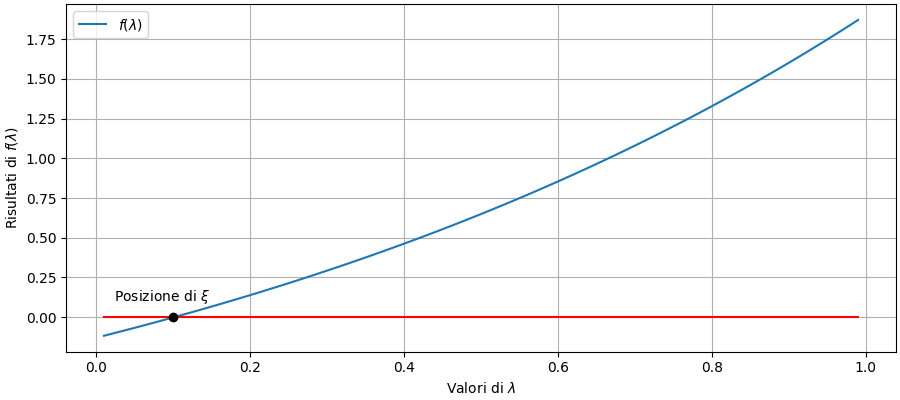
\includegraphics[width=\linewidth]{assets/image-002.png}
    \end{center}
\end{example}

Come abbiamo potuto notare dall'esempio, grazie ai tre metodi possiamo trovare una posizione approssimativa delle varie radici di una funzione. Ma come mai ci interessa tanto sapere la posizione di dove la funzione cambia segno? Perché grazie al \textbf{teorema di Bolzano}, questo ci permette di localizzare una radice.

\begin{theorem}{Teorema di Bolzano}
    Dato un \textbf{intervallo} $[a, \; b]$ e una \textbf{funzione} $f(x)$ \textbf{continua}, se $f(a)$ ha \textbf{segno discorde} rispetto a $f(b)$ (quindi, se $f(a) \cdot f(b) < 0$), allora $f(x)$ \textbf{interseca almeno una volta} l'asse delle $x$
\end{theorem}

È importante tuttavia sapere anche restringere l'intervallo di osservazione delle radici. Supponiamo di avere in esame la funzione
\[ p(x) \eq x^4 + 2x^3 + 7x^2 - 11 \eq 0 \]

mostriamo qui due grafici della funzione, in intervalli diversi:
\begin{center}
    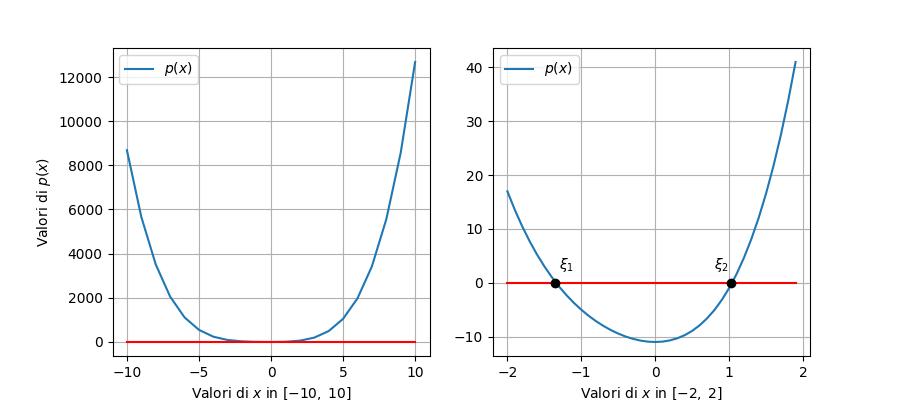
\includegraphics[width=\linewidth]{assets/image-003.png}
\end{center}

Notiamo come, in base all'intervallo, è più semplice notare la posizione delle radici. Infatti, $p(x)$ ha 4 radici, di cui due reali e due complesse coniugate.

\section{Metodo di Bisezione (o Dicotomico)}

Tra i vari metodi utilizzabili per trovare le radici in una funzione, il più semplice e immediato da utilizzare è il \textbf{metodo di bisezione}, o \textbf{metodo dicotomico}. Questo metodo permette, una volta individuato un intervallo di separazione in cui si trova una \textbf{singola radice}, di costruire una successione $\{ x_k \}$ di approssimazioni di $\xi$. Per applicare dunque questo metodo vanno rispettate due condizioni, dette \textbf{ipotesi di applicabilità}:
\begin{itemize}
    \item è stato individuato un intervallo $I \eq [a, \; b]$, all'interno del quale è presente \textbf{un'unica radice} $\xi$;
    \item la funzione $f$ in esame deve essere \textbf{continua in} $I$ (formalmente, $f \in C^0 [a, \; b]$, dove $C^0$ è l'insieme di funzioni continue);
    \item i due estremi $a$ e $b$ devono avere \textbf{segno discorde} (dunque $f(a) \cdot f(b) < 0$).
\end{itemize}

In sintesi, il teorema di Bolzano deve essere rispettato all'interno del nostro intervallo $I$; il metodo di bisezione infatti usa estensivamente il suddetto teorema. Passiamo dunque ad esaminare l'algoritmo del metodo di bisezione:

\begin{algorithm}[H]
    \caption{Metodo di bisezione (o dicotomico)}
    \KwIng{L'intervallo $[a, b]$, la funzione $f(x)$ e la tolleranza}
    $a \gets a_0, \; b \gets b_0$\;
    $\xi_{\text{seq}} \gets \{\}$ \tcp*{$\xi_{\text{seq}}$ è una sequenza vuota}
    \For{$k$ in $1, \; 2, \; 3, \; ...$}{
        $x_k \gets \frac{a + b}{2}$\;
        $d \gets |x_k - x_{k - 1}|$\;
        \BlankLine
        Add $x_k$ to $\xi_{\text{seq}}$\;
        \BlankLine
        \tcp{Se si trova la radice oppure viene raggiunta la tolleranza, l'algoritmo si ferma}
        \If{$(f(x_k) = 0)$ \textbf{or} $(d < \text{tol})$}{
            \textbf{return} $\xi_{\text{seq}}$
        }
        \BlankLine
        \tcp{In base all'intervallo che contiene la radice, ripetere l'algoritmo con l'intervallo aggiornato}
        \If{$f(a) \cdot f(x_k) < 0$}{
            $a \gets a, \; b \gets x_k$
        }
        \BlankLine
        \If{$f(x_k) \cdot f(b) < 0$}{
            $a \gets x_k, \; b \gets b$
        }
    }
\end{algorithm}

\nwl
Per il metodo di bisezione, l'idea è che dato un intervallo $I = [a, \; b]$, \textbf{dividendo} $I$ sempre \textbf{in sotto-intervalli} più contenuti, riusciremmo eventualmente ad ottenere un intervallo più piccolo all'interno del quale troveremmo la nostra radice $\xi$. Ogni sotto-intervallo è costituito da una delle due metà di $I$. Per sapere quale sotto-intervallo contiene $\xi$, basta applicare il teorema di Bolzano. L'algoritmo è semplice, e genera una successione di tutte le approssimazioni di $\xi$, denominata $\{x_k\}$ (o, nell'algoritmo, $\xi_{\text{seq}}$). La precisione del metodo di bisezione è ottenibile calcolando il relativo \textbf{errore di troncamento}.

\begin{definition}{Errore di troncamento}
    L'\textbf{errore di troncamento} è l'errore commesso \textbf{approssimando} la radice $\xi$ con il $k$-esimo elemento della successione creata tramite l'algoritmo del metodo di bisezione
    \[ e_k \eq \xi - x_k \]
\end{definition}

Ma l'algoritmo \textbf{può convergere}? Intuitivamente, convergerà verso $\xi$ solo se l'errore si dovesse ridurre a 0. Formalmente, possiamo esprimere questa relazione come
\[ \lim_{k \to \infty} x_k \eq \xi \quad \Longleftrightarrow \quad \lim_{k \to \infty} |e_k| \eq 0 \]

Possiamo però esprimere $e_k$ anche in altri termini. Per il metodo di bisezione, noi sappiamo che alla $k$-esima iterazione, $\xi$ sarà presente solo in $[a_{k - 1}, \; x_k]$ o in $[x_k, \; b_{k - 1}]$.

\begin{center}
    \begin{tikzpicture}
        \draw[black, thick] (0, 0) -- (8, 0);
        \fill[blue] (0, 0) circle (2pt) node [below] {$a_{k - 1}$};
        \fill[blue] (4, 0) circle (2pt) node [below] {$x_k$};
        \fill[blue] (8, 0) circle (2pt) node [below] {$b_{k - 1}$};
        \fill[red] (5.5, 0) circle (2pt) node [below] {$\xi$};
    \end{tikzpicture}
\end{center}

Dunque, data una generica iterazione $x_k$, l'errore di troncamento alla suddetta sarà uguale a
\[ |e_k| < \frac{b_{k - 1} - a_{k - 1}}{2} \]

Ora, siccome l'intervallo $[a_{k - 1}, \; b_{k - 1}]$ ha ampiezza pari alla metà dell'intervallo all'iterazione precedente (dunque $[a_{k - 2}, \; b_{k - 2}]$), possiamo costruire anche una formula generica dell'errore per qualsiasi iterazione $k$:
\[ |e_k| < \frac{b_{k - 1} - a_{k - 1}}{2} = \frac{b_{k - 2} - a_{k - 2}}{2^2} \eq \; ... \; \eq \frac{b - a}{2^k} \]

Dunque, anche il limite di prima può essere riscritto come
\[ 0 \leq \lim_{k \to \infty} |e_k| < \lim_{k \to \infty} \frac{b - a}{2^k} = 0 \]

\subsection{Ordine di corvengenza e Criteri di arresto}

Abbiamo visto che il metodo di bisezione converge, ma è anche importante che converga in tempi rapidi. Come possiamo determinare la "velocità" di convergenza? Questo viene determinato in base a un valore chiamato \textbf{ordine di convergenza} $p$.

\begin{definition}{Ordine e Fattore di Convergenza}
    Sia $\{ x_k \}$ una successione di approssimazioni \textbf{convergente} a $\xi$. Si dice che la successione ha un \textbf{ordine di convergenza} $p$ e un \textbf{fattore di convergenza} $C$ se esistono due numeri reali $p \geq 1$ e $C > 0$ tali che
    \[ \lim_{k \to \infty} \frac{|e_{k + 1}|}{|e_k|^p} \eq C \]

    Se $p \eq 1$, si dice che la convergenza è \textbf{lineare}, se $p \eq 2$, si dice invece che la convergenza è \textbf{quadratica}.
\end{definition}

Applicando la definizione di ordine e fattore di convergenza al metodo di bisezione, otteniamo che, per $k \to \infty$, si ha:
\[ \frac{|e_{k + 1}|}{|e_k|^p} \eq \frac{\frac{b - a}{2^{k + 1}}}{\frac{b - a}{2^k}} \eq \frac{2^k}{2^{k + 1}} \eq \frac{2^k}{2^k} \cdot \frac{1}{2} \eq \frac{1}{2} \]

Cosa ci dice il risultato appena ottenuto? Che, supponendo una convergenza lineare, otteniamo un fattore di convergenza di $\nicefrac{1}{2}$. Questo ci dice che la convergenza è in realtà \textbf{lenta}: ad ogni step dell'algoritmo riusciamo a dimezzare l'errore, e guadagnamo una cifra binaria per meglio esprimere il nostro risultato. Siccome $2^{-4} < 10^{-1} < 2^{-3}$, allora ogni 3 o 4 iterazioni si riesce a guadagnare una cifra decimale.
\nwl
Tuttavia, a causa degli errori di arrotondamento e troncamento da parte del computer, è praticamente impossibile che si riesca a raggiungere $f(x_k) \eq 0$. Dunque, quando dovremmo interrompere i calcoli? Possiamo definire dei \textbf{criteri di arresto a posteriori}, ovverosia
\[ \begin{cases}
|e_k| \simeq |x_k - x_{k - 1}| < \epsilon & \text{Se l'errore diventa minore di una tolleranza } \epsilon ... \\
|f(x_k)| < \epsilon & \text{...o se la funzione ritorna numeri minori della tolleranza } \epsilon
\end{cases} \]

Nel caso dell'algoritmo di bisezione, è stato scelto in precedenza di usare il primo criterio, ma potevano essere usati entrambi i criteri. Possiamo anche calcolare \textbf{a priori} una stima di quante iterazioni $K$ avremo bisogno prima di ottenere un errore minore di $\epsilon_{\text{min}}$. Per farlo, ci avvaliamo della formula dell'errore di troncamento:
\[ |e_k| < \frac{b - a}{2^k} < \epsilon_{\text{min}} \quad \Longrightarrow \quad K > \frac{\log(b - a) - \log(\epsilon_{\text{min}})}{\log(2)} \]

$K$ dovrà essere arrotondato all'intero più vicino, in quanto deve essere un intero positivo.

\section{Metodo di Newton-Raphson}

Forse uno dei metodi più utilizzati quando si parla di equazioni non lineari, il \textbf{metodo di Newton-Raphson} (o metodo delle tangenti) è un metodo molto usato, grazie alla sua convergenza più immediata rispetto al metodo di bisezione. Questo metodo prevede di approssimare una funzione $f(x)$ in un intorno $I$, all'interno del quale si deve trovare una e una sola radice $\xi$, grazie alle sue \textbf{tangenti} in vari punti, le quali vengono calcolate grazie ad uno \textbf{sviluppo in serie di Taylor}.
\nwl
Partendo da un'approssimazione iniziale della radice, che chiameremo $x_0$, è possibile costruire la tangente $t_0$ alla funzione nel punto di intersezione tra $x = x_0$ e la funzione stessa (quindi, nel punto $(x_0, \; f(x_0))$). Per costruire la tangente, viene utilizzato lo sviluppo in serie di Taylor (\textbf{fino al primo ordine}), che tramite il calcolo della derivata prima permette di trovare l'equazione di $t_0$:
\[ t_0 \eq f(x_0) + f'(x_0) \cdot (x - x_0) \]

Calcolata la tangente, si procede recuperando il punto di intersezione tra $t_0$ e l'asse delle $x$; tale punto viene chiamato $x_1$. Una volta ottenuto $x_1$, il procedimento ricomincia da capo: si trova dunque il punto di intersezione $(x_1, \; f(x_1))$, si calcola la tangente $t_1$ nel punto appena trovato (quindi $t_1 \eq f(x_1) + f'(x_1) \cdot (x - x_1)$) e si ottiene un nuovo punto, chiamato $x_2$. Il procedimento continua finché non si raggiunge o la radice o un criterio d'arresto.
\nwl
Generalmente, ad ogni iterazione $k \eq 1, \; 2, \; ...$ del metodo, la nuova approssimazione della radice $x_k$ è data dall'intersezione tra la tangente $t_k$ a $f(x)$ nel punto $(x_{k - 1}, \; f(x_{k - 1}))$ e l'asse delle $x$:
\[ t_{k} \eq f(x_k) + f'(x_k) \cdot (x - x_k) \quad \Longrightarrow \quad \text{si vuole risolvere} \quad f(x_k) + f'(x_k) \cdot (x - x_k) \eq 0 \]

\begin{center}
    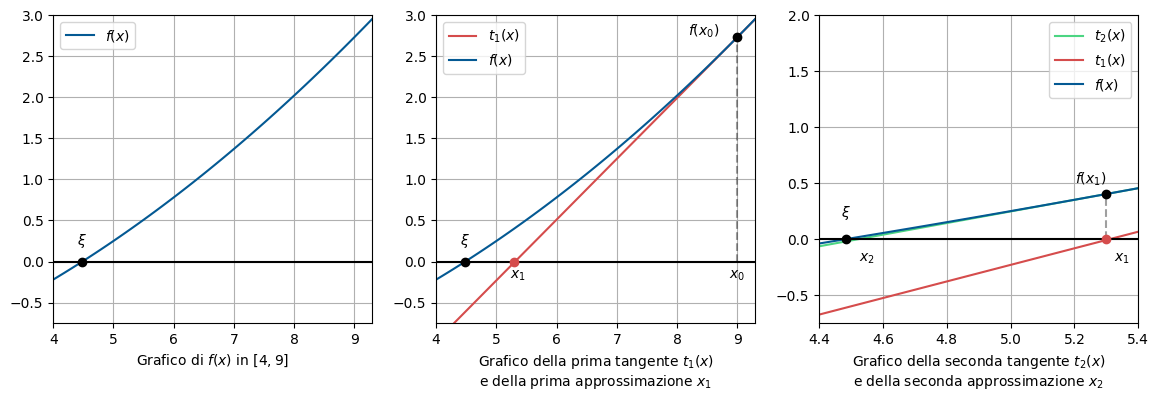
\includegraphics[trim=0 0 0 0, clip=false, width=\textwidth]{assets/image-004.png}
\end{center}

Possiamo tuttavia rifattorizzare l'espressione, così da renderla in funzione dell'approssimazione in un'iterazione $k$:
\begin{align*}
    f(x_{k - 1}) + f'(x_{k - 1}) \cdot (\underbrace{x}_{\text{becomes } x_k} - x_{k - 1}) &\eq 0 \\
    f(x_{k - 1}) + x_k \cdot f'(x_{k - 1}) - x_{k - 1} \cdot f'(x_{k - 1}) &\eq 0 \\
    -x_k \cdot f'(x_{k - 1}) &\eq f(x_{k - 1}) - x_{k - 1} \cdot f'(x_{k - 1}) \\
    -x_k &\eq \frac{f(x_{k - 1})}{f'(x_{k - 1})} - x_{k - 1} \cdot \frac{f'(x_{k - 1})}{f'(x_{k - 1})} \\
    x_k &\eq x_{k - 1} - \frac{f(x_{k - 1})}{f'(x_{k - 1})}
\end{align*}

L'algoritmo, dal punto di vista matematico, diventa dunque il seguente:
\[ \begin{cases}
    x_0 & \text{viene dato come input} \\
    x_k \eq x_{k - 1} - \frac{f(x_{k - 1})}{f'(x_{k - 1})} & \text{per } k \eq 1, \; 2, \; ...
\end{cases} \]
\nwl
Viene qui mostrato l'algoritmo del metodo:
\nwl
\begin{algorithm}[H]
    \caption{Metodo di Newton-Raphson (o delle tangenti)}
    \KwIng{La funzione $f(x)$, un'approssimazione iniziale $x_0$ e la tolleranza}
    $x_k \gets x_0$\;
    $\xi_{\text{seq}} \gets \{\}$\;
    \BlankLine
    \tcp{Finché $x_k$ non è uguale a $\xi$ oppure finché non si raggiunge la tolleranza...}
    \While {$(f(x_k) \neq 0)$ \textbf{or} $(x_k > \text{tol})$}{
        \tcp{...calcola la nuova approssimazione di $\xi$}
        $x_{k + 1} \gets x_k - \frac{f(x_k)}{f'(x_k)}$\;
        Add $x_{k + 1}$ to $\xi_{\text{seq}}$\;
        $x_k \gets x_{k + 1}$\;
    }
    \BlankLine
    \textbf{return} $x_k$, $\xi_{\text{seq}}$
\end{algorithm}


\end{document}
